\chapter{Métricas}

\section{Processo de Medição}

Medição é o mapeamento de relações empíricas em relações formais. Isto é, 
quantificação em símbolos com objetivo de caracterizar uma entidade por meio de 
seus atributos. \cite{Fenton98}.
	
Segundo \citeonline{ISO:15939}, medição, que é uma ferramenta primordial para 
gerenciar as atividades do desenvolvimento de software e para avaliar a 
qualidade dos produtos e a capacidade de processos organizacionais, é um 
conjunto de operações que visam por meio de um objeto determinar um valor a uma 
medida ou 
métrica.\footnote{A definição formal da \citeonline{ISO:15939} não utiliza o 
termo métrica, sendo que este é definido pelo GQM em \citeonline{Basili96b}, 
que é uma outra abordagem para medição, contudo compreende-se que o termo medida 
tem valor semântico equivalente ao de métrica no contexto do presente trabalho}. 
	
	
O processo de medição da \citeonline{ISO:15939}, como é mostrado na figura 
\ref{processo}, que fora extraído de \citeonline{Gava2006}, consiste de quatro 
atividades que são sequenciadas em um ciclo iterativo, permitindo feedback e 
melhoria contínua do processo. Trata-se de uma adaptação do ciclo 
PDCA (Plan-Do-Check-Act), comumente utilizado como base para a melhoria da 
qualidade \cite{Barcellos2010}.  O processo visa a construção de produtos de 
informação para cada necessidade seguindo um modelo de informação, que é 
mostrado na figura \ref{informação}.
		
\begin{figure}[h]
\centering	
	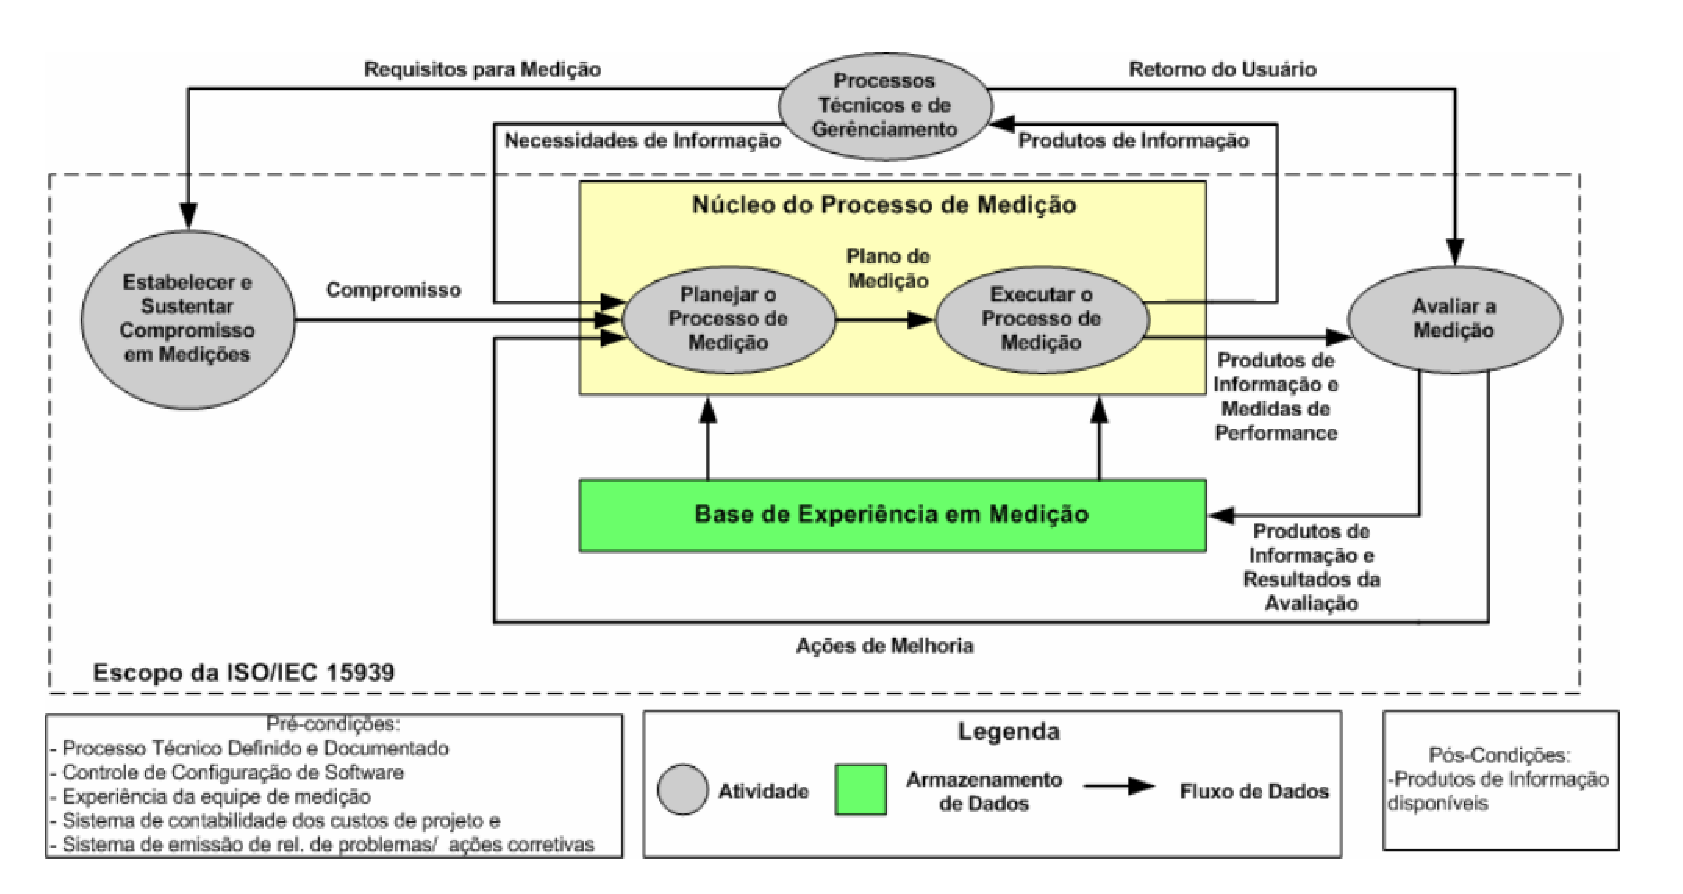
\includegraphics[keepaspectratio=true,scale=0.45]{figuras/processo15939.eps}
	\caption{Processo de Medição da ISO 15939}
	\label{processo}
\end{figure}
		

\begin{figure}[h]
\centering
	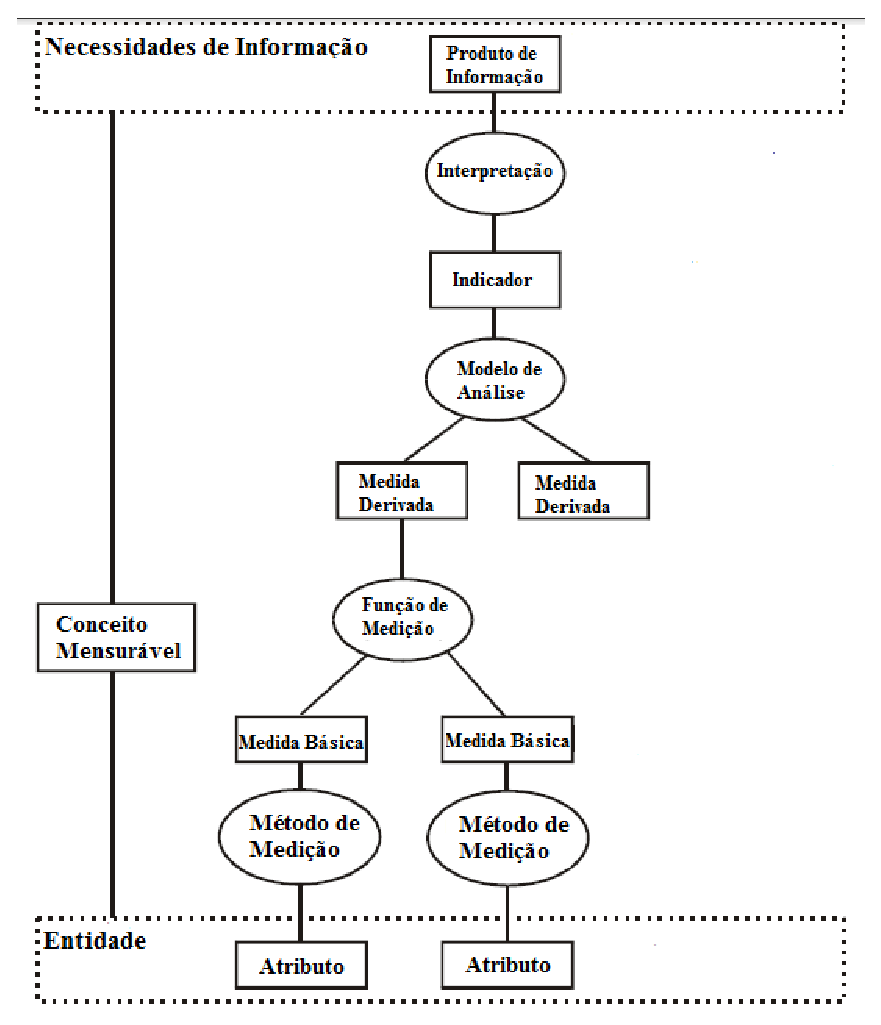
\includegraphics[keepaspectratio=true,scale=0.55]{figuras/modelo15939.eps}
	\caption{Modelo de Informação da ISO 15939}
	\label{informação}
\end{figure}

A terminologia do modelo de informação, que é mostrado na figura 
\ref{informação} é descrito a seguir:

\begin{description}
	%----------
	\item [Necessidade de Informação.]  São situações as quais requer 
	 conhecimento de uma ou mais entidades para gerenciar objetivos, metas, 
	 riscos e problemas.
	
	%---------
	 \item [Entidade.]  Uma entidade é um objeto (como por exemplo, um processo,
	 produto, projeto ou recurso) que é caracterizado por um atributo 
	 mensurável;
	 
	%----------
	 \item [Atributo.]  Um atributo é uma propriedade ou característica de uma 
	 entidade que pode distinguí-la quantitativamente ou qualitativamente 
	 utilizando métodos manuais ou automáticos
	
	%----------
	 \item [Conceito Mensurável.]  Uma relação entre os atributos e as 
	 necessidades de informação. Como por exemplo, a qualidade de um produto. 
	 
	%----------
	 \item [Medida Básica ou Métrica Direta.] Uma medida básica é definida em 
	 termos do atributo e do método para sua quantificação, ou seja, é a 
	 variável a qual se atribui um valor. Cada medida básica é funcionalmente 
	 independente de outras medidas básicas e captura apenas um atributo. 
	%----------
	 \item [Método de Medição.] O método de medição é uma sequência de 
	 operações, descritas genericamente, usadas qualificar ou quantificar um 
	 atributo, ou seja, obter uma medida básica ou derivada com respeito a uma 
	 escala. Um método de medição pode ser classificado em:
	
		\begin{description}
		 \item [Subjetivo.] Envolve o julgamento humano. Resulta em medidas ou 
		 métricas subjetivas.
		 \item [Objetivo.] Baseado em regras numéricas, tais como contagem. 
		 Pode ser realizado de forma manual ou automática. Resulta em medidas 
		 ou métricas objetivas.
		\end{description}
	%----------
	 \item [Escala.] Uma escala é um conjunto ordenado de valores, contínuos ou 
	 discretos, ou uma série de categorias as quais um atributo é mapeado. 
	 O método de medição mapeia a magnitude, ou valor absoluto, de um atributo 
	 medido em um valor de escala. As escalas podem ser: 
	
		\begin{description}
			%----------
		 	\item [Nominal.] A medição é categórica. Por exemplo, a 
			classificação dos tipos de defeitos. Nesta escala, só é possível 
			realização de comparações.
			%----------
			\item [Ordinal.] A medição é baseada em ordenação. Por exemplo, a 
			classificação de atletas de uma prova de atletismo.
			%----------
		 	\item [Intervalo.] A medição é baseada em distâncias iguais 
			definidas para as menores unidade. Por exemplo, o aumentar de 1º C 
			de um termômetro. Nesta escala é possível realizar ordenação, soma 
			e subtração.
			%----------
		 	\item [Racional.] A medição é baseada em distâncias iguais definidas 
			para as menores unidades, e neste caso é possível a ausência por 
			meio do zero absoluto. Como por exemplo, a quantidade de linhas de 
			código em uma classe. Nesta escala, é possível realizar ordenação, 
			soma, subtração, multiplicação e divisão.

		\end{description}
	%----------
	 \item [Função de Medição.] Trata-se do algoritmo para combinar duas ou mais 
	 medidas básicas ou métricas diretas.
	%----------
	 \item [Medida Derivada ou Métrica Derivada.] Uma medida derivada ou métrica 
	 derivada é definida como uma função de medição de duas ou mais medidas 
	 básicas ou métricas diretas.
	
	 \item [Indicador.]  É uma medida que fornece uma estimativa ou avaliação de 
	 atributos especificados em relação a uma necessidade de informação. 
	 Um indicador inclui um ou mais valores de medidas básicas e/ou derivadas.

	\item [Interpretação.]  É a explicação dos indicadores, isto é, a 
	interpretação que cada valor quantitativo do indicador mostra.
	
	\item [Produto de Informação] É o resultado esperado do processo de medição, 
	que visa responder as necessidades de informação. O produto de informação 
	pode vir a se materializar em forma de relatórios, gráficos ou planilhas.
\end{description}






%---------------------------------------------------------------------------------------------------------------------%
\section{Classificação das Métricas}	
\label {Classificação das Métricas}
O modelo proposto pela \citeonline{ISO:15939} concentra-se na identificação da 
necessidade de informação sobre alguma entidade (processo ou projeto). Daí advém
a forma mais genérica de classificação, quanto a objeto da métrica, que divide 
as métricas de software em: \textit{métricas de processo} e 
\textit{métricas de produto} \cite{Mills:1999}. Ainda é possível, segundo a 
\citeonline{ISO:15939}, dividir as métricas quanto ao método de medição, podendo
estas serem \textit{métricas objetivas} ou \textit{métricas subjetivas}.


Segundo o modelo de qualidade da \citeonline{ISO25023} 
(Fig. \ref{modelodequalidade}), as métricas de produto podem ser subdivididas 
em três categorias :
				
\begin{figure}[h]
\centering
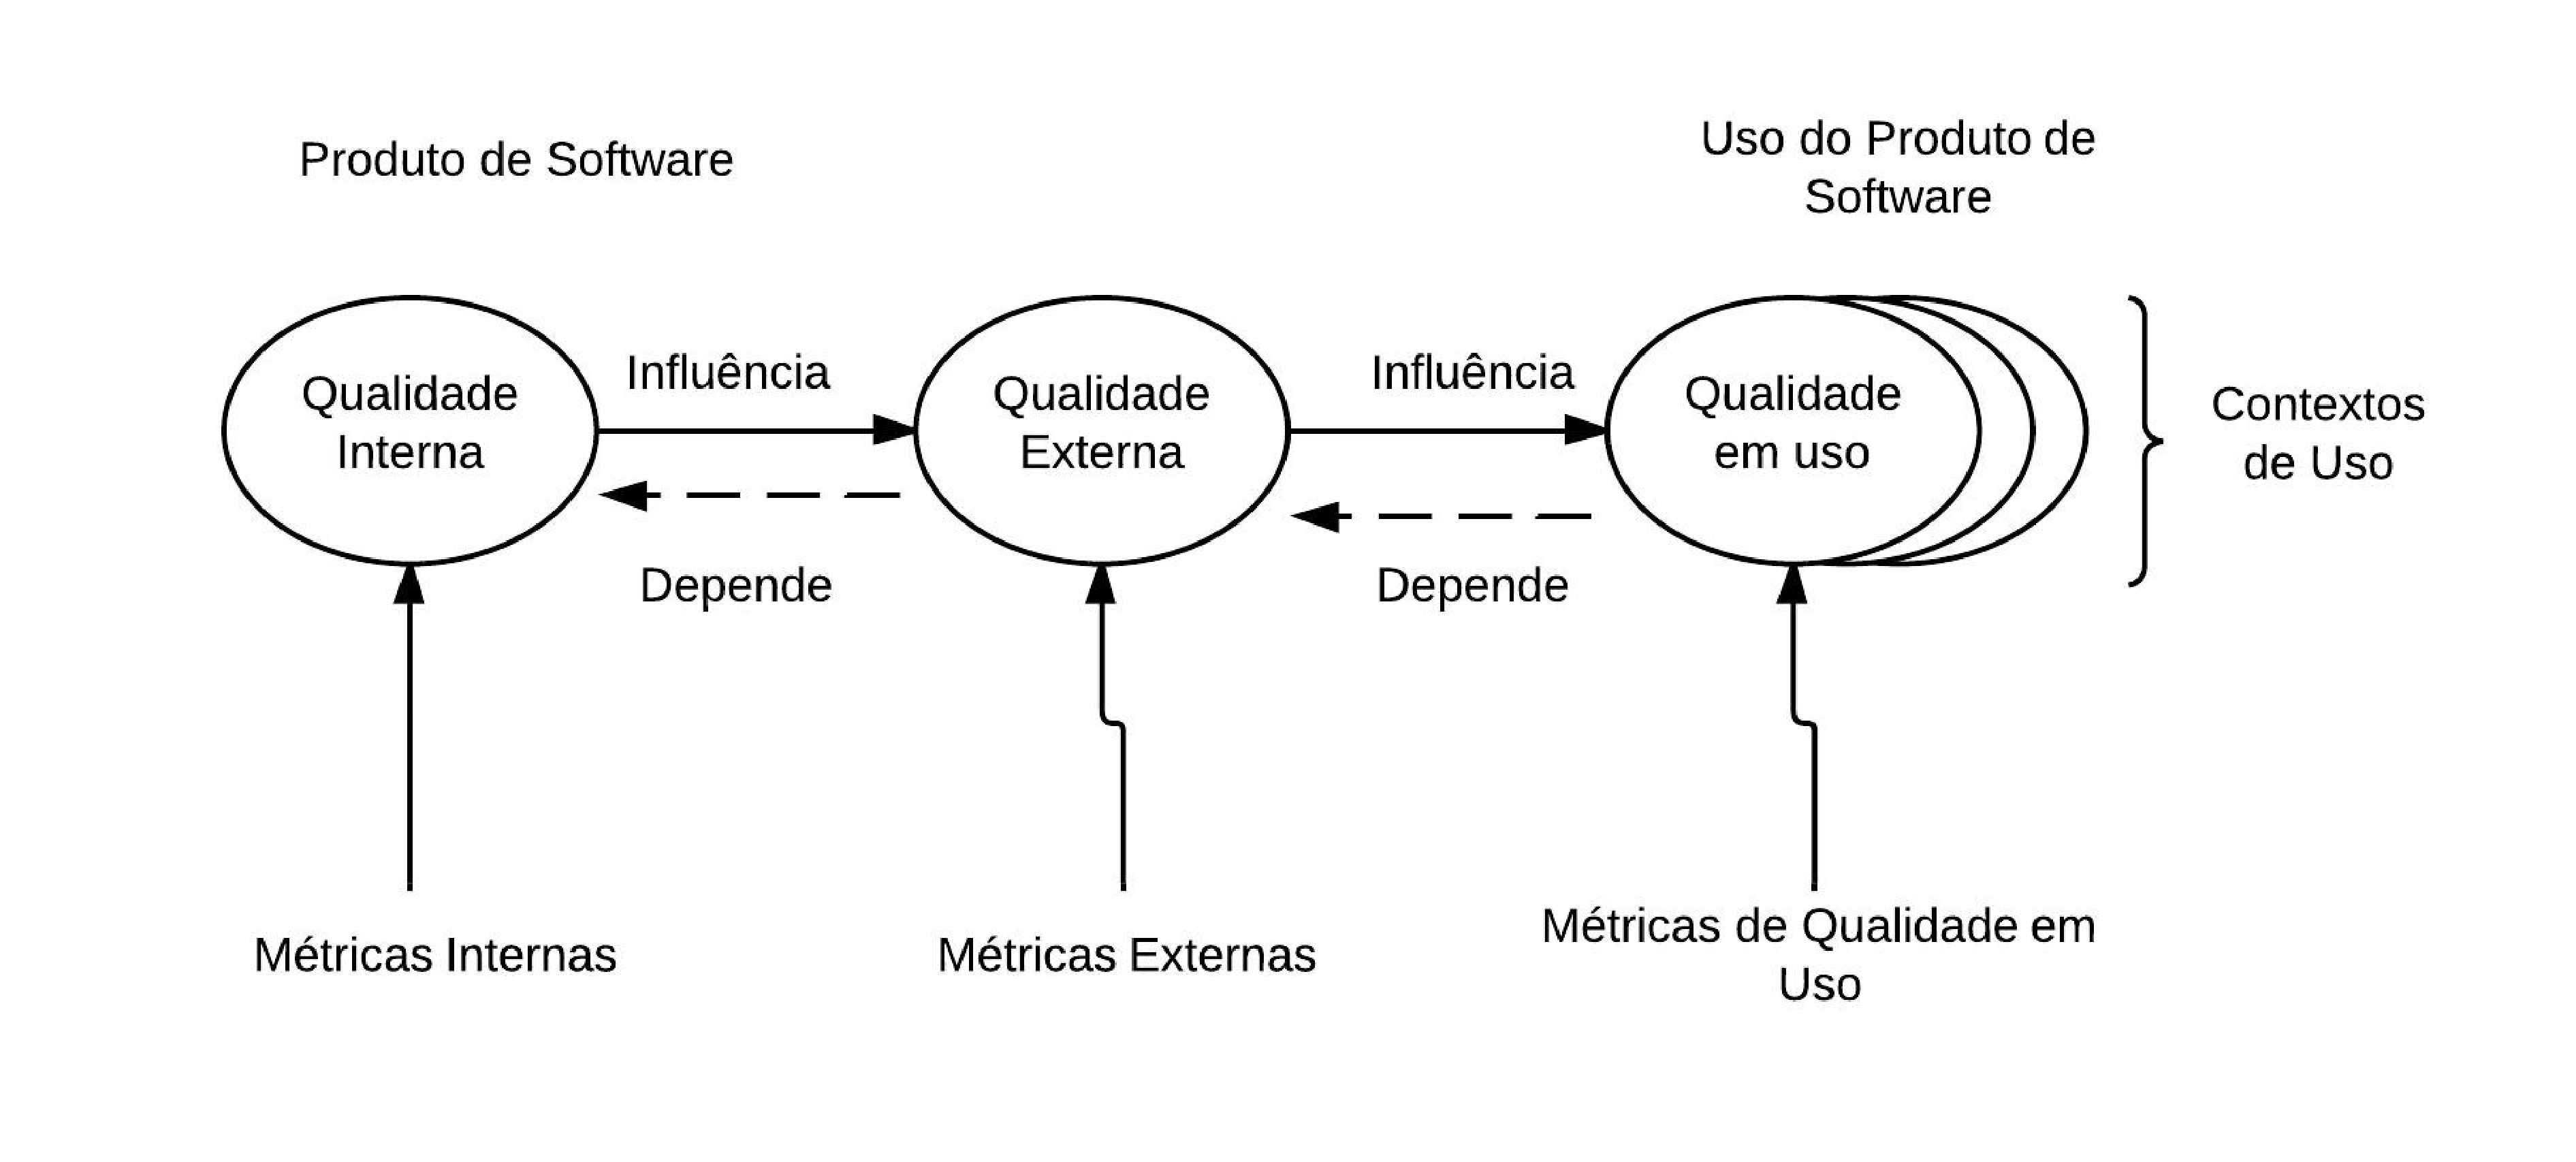
\includegraphics[keepaspectratio=false,scale=0.7]{figuras/modelodequalidade.eps}
\caption{Modelo de Qualidade do Produto da ISO 25023}
\label{modelodequalidade}
\end{figure}
			
\begin{description}
%-----------------------------
		\item[Métricas Internas.] 
		São métricas que aferem a qualidade interna do software por meio da 
		avaliação de estruturas internas que compõem o software em estágio de 
		desenvolvimento. São conhecidas como métricas de código-fonte.

%-----------------------------			
		\item[Métricas Externas.]
		São métricas que capturam o comportamento do software. Exemplos de 
		atributos da qualidade externa: correção, usabilidade, eficiência e 
		robustez. qualidade externa mede  o comportamento do software. Estas só 
		podem ser aferidas por atividades de teste do desenvolvimento do 
		software em condições similares as que serão encontradas em ambientes de
		implantação.

%-----------------------------			
		\item[Métricas de Qualidade em Uso.]
		 São métricas que aferem se o software atende as necessidades do cliente
		 com eficiência, produtividade, segurança e satisfação em contextos 
		 específicos de uso. Estas só podem ser coletadas em ambientes reais, 
		 isto é, o ambiente o qual fora previamente projetado.
			 
\end{description}
		
				

%---------------------------------------------------------------------------------------------------------------------%
\section {Métricas de Código-Fonte}
\label {Métricas de Código-Fonte}

Segundo a chamada de trabalhos do SCAM 2013~\footnote{13th IEEE International 
Working Conference on Source Code Analysis and Manipulation}, código-fonte é 
qualquer descrição completamente executável de um sistema de software, desde de 
linguagem de máquina até representações gráficas executáveis.

As métricas internas de produto ou métricas de código fonte são obtidas por meio
da análise das estruturas internas do código sem realizar sua execução 
\cite{Wichmann95}  \cite{Nielson:1999} \cite{Sommerville10}. Popularmente, o 
termo análise estática de código se refere à uma análise automatizada de 
obtenção de métricas de código fonte \cite{Terra2008} 
\cite{Emanuelsson2008}.

As métricas de código-fonte são métricas objetivas e tem características como 
validade, simplicidade, objetividade, fácil obtenção e robustez \cite{Mills:1999}. 
\citeonline{Meirelles2013} realizou um levantamento sistemático na literatura 
das métricas de código-fonte. Estas foram categorizadas, nas seguintes 
categorias:


	\begin{description}
	\item [Tamanho e Complexidade.] O tamanho do código-fonte foi uma das 
	primeiros conceitos mensuráveis do software, dado que o software poderia 
	ocupar espaço tanto em forma de cartões perfurados quanto em forma de papel 
	quando o código-fonte é impresso. A segunda lei de \citeonline{Lehman1980b} 
	enuncia que a complexidade aumenta à medida que o software é evoluído, 
	a menos que seja um trabalho de manutenção. Logo é perceptível que as 
	métricas de complexidade estão diretamente ligadas as métricas de tamanho, 
	sendo a modificação em uma provavelmente impactará na outra, por este motivo,
	a seção \ref{métricas tamanho e complexidade} apresenta as métricas de tamanho e
	complexidade.
	

%-----------------------------
	\item [Orientação à Objetos.] A evolução dos paradigmas de programação 
	permitiu que as linguagens de programação, assumissem diversas 
	características entre si. O paradigma funcional, por exemplo, enxerga o 
	programa como uma sequência de funções que podem ser executadas em modo 
	funcional. Já o paradigma orientado a objetos visa abstrair as unidades 
	computacionais em Classes, que representam em grande parte do 
	desenvolvimento unidades reais, e partir destas abstrair instâncias 
	computacionais, isto são, objetos propriamente ditos. Para cada paradigma, 
	são necessárias métricas específicas. A seção \ref{métrica objetos} 
	apresenta algumas das métricas do paradigma orientado a objetos, pois este 
	ainda é o paradigma mais utilizado no mercado de desenvolvimento de 
	software. 
	\end{description}
	

%-----------------------------------------------------------------------------------------------------------------------------
\subsection{Métrica de Tamanho e Complexidade}
\label{métricas tamanho e complexidade} 
	
\begin{description}

	\item[LOC (\textit{Lines of Code})] \textbf{Número de Linhas de Código} 
	foi uma das primeiras métricas utilizadas para medir o tamanho de um 
	software. São contadas apenas as linhas executáveis, ou seja, são excluídas 
	linhas em branco e comentários. Para efetuar comparações entre sistemas 
	usando LOC, é necessário que ambos tenham sido feitos na mesma linguagem de 
	programação e que o estilo esteja normalizado \cite{Jones91}.
	
	\item[ACCM (\textit{Average Cyclomatic Complexity per Method})] \textbf{
	Média da Complexidade Ciclomática por Método} mede a complexidade do métodos
	ou funções de um programa. Essa métrica pode ser representada através de um 
	grafo de fluxo de controle \cite{McCabe76}. O uso de estruturas de controle,
	tais como, \textit{if, else, while} aumentam a complexidade ciclomática de 
	um de um método.

\end{description}




\subsection{Métricas de Orientação à Objetos}
\label{métrica objetos}

\begin{description}

	\item[ACC (\textit{Afferent Connections per Class})] 
	\textbf{Conexões Aferentes por Classe} é número total de classes externas de 
	um pacote que dependem de classes de dentro desse pacote. Quando calculada 
	no nível da classe, essa medida também é conhecida como \textit{Fan-in} da 
	classe, medindo o número de classes das quais a classe é derivada e, assim, 
	valores elevados indicam uso excessivo de herança múltipla \cite{McCabe94} 
	\cite{Chidamber94}.
	
	
	%-----------------------------
	\item[RFC (\textit{Response For a Class})] \textbf{Respostas para uma 
	Classe} é número de métodos dentre todos os métodos que podem ser invocados 
	em resposta a uma mensagem enviada por um objeto de uma classe 
	\cite{Sharble93}.
	
	\item[LCOM4 (\textit{Lack of Cohesion in Methods})] \textbf{Falta de Coesão
	entre Métodos}. Originalmente proposto por \citeonline{Chidamber94} 
	como LCOM, contudo essa não teve uma grande aceitabilidade. Após críticas e 
	sugestões a métrica revisada por \citeonline{LCOM4}, que propôs a LCOM4. 
	Para calcular LCOM4 de um módulo, é necessário construir um gráfico 
	não-orientado em que os nós são os métodos e atributos de uma classe. Para 
	cada método, deve haver uma aresta entre ele e um outro método ou variável 
	que ele usa. O valor da LCOM4 é o número de componentes fracamente 
	conectados nesse gráfico. 

	
	%-----------------------------
	\item[NOM (\textit{Number of Methods})] \textbf{Número de Métodos} é usado 
	para medir o tamanho das classes em termos das suas operações implementadas. 
	Essa métrica é usada para ajudar a identificar o potencial de reúso de uma 
	classe. Em geral, as classes com um grande número de métodos são mais 
	difíceis de serem reutilizadas, pois elas são propensas a serem menos coesa
	\cite{Lorenz94}.
	

	%-----------------------------
	\item [DIT (\textit{Depth of Inheritance Tree})] \textbf{Profundidade da 
	Árvore de Herança} é o número de superclasses ou classes ancestrais da 
	classe sendo analisada. São contabilizadas apenas as superclasses do sistema, 
	ou seja, as classes de bibliotecas não são contabilizadas. Nos casos onde 
	herança múltipla é permitida, considera-se o maior caminho da classe até uma
	das raízes da hierarquia. Quanto maior for o valor DIT, maior é o número de 
	atributos e métodos herdados, e portanto maior é a complexidade 
	\cite{Shih97}.
	
	\item[NOC (\textit{Number of Children})] \textbf{Número de Filhos} é o 
	número subclasses ou classes filhas que herdam da classe analisada 
	\cite{Rosenberg97}. Deve se ter cautela ao modificar classes com muitos 
	filhos, pois uma simples modificação de assinatura de um método, pode criar
	uma mudança em muitas classes.
	

\end{description}
	
\subsection{Intervalos da Métricas}
\label{Intervalos das Métricas}
Em sua tese \citeonline{Meirelles2013} analisou as métricas do código-fonte de 
38 projetos de software livre, em um total de 344.872 classes das aplicações 
mais bem sucedidas (\textit{Chrome, Firefox, OpenJDK, VLC e entre outros}) e 
percebeu que há certos valores que são frequentemente encontrados quando se 
analisa o código-fonte de aplicações que utilizam a mesma linguagem de 
programação. \citeonline{Meirelles2013} classifica estes intervalos, em 
\textit{muito frequente, frequente, pouco frequente e não frequente}. Visando o 
o melhor entendimento das métricas, resolveu-se renomear tal como a tabela 
\ref{nomes}. Posteriormente, é apresentada a tabela \ref{metrics}, decorrente do
estudo de \citeonline{Meirelles2013}, com os intervalos encontrados para C++ e 
Java.

	\begin{table}[!ht]
	\begin{center}
	 \begin{tabular}{|l|l|}
		\hline
		Intervalo de Frequência & Intervalo Qualitativo \\ \hline
		Muito Frequente & Excelente \\ \hline
		Frequente       & Bom       \\ \hline
		Pouco Frequente & Regular   \\ \hline
		Não Frequente   & Ruim      \\ \hline
		\end{tabular}
		\caption{Nome dos Intervalos de Frequência}
		\label{nomes}
		\end{center}
		\end{table}

	\begin{table}[!ht]
	\begin{center}
	\begin{tabular}{ |l|l|l|l| }
		\hline
		Métrica & Indicador & Java & C++ \\ \hline
		%-------------------------------
		\multirow{4}{*}{LOC} 
		 & Excelente & [de 0 a 33] & [de 0 a 31] \\
		 & Bom & [de 34 a 87] & [de 32 a 84] \\
		 & Regular & [de 88 a 200] & [de 85 a 207] \\
		 & Ruim & [acima de 200] & [acima de 207] \\ \hline
		 %---------------------------------
		 
		 %-------------------------------
		\multirow{4}{*}{ACCM} 
		 & Excelente & [de 0 a 2,8] & [de 0 a 2,0] \\
		 & Bom & [de 2,9 a 4,4] & [de 2,1 a 4,0] \\
		 & Regular & [de 4,5 a 6,0] & [de 4,1 a 6,0] \\
		 & Ruim & [acima de 6] & [acima de 6] \\ \hline
		 %---------------------------------
		 
		 
		%-------------------------------
		\multirow{4}{*}{ACC} 
		 & Excelente & [de 0 a 1] & [de 0 a 2,0] \\
		 & Bom & [de 1,1 a 5] & [de 2,1 a 7,0] \\
		 & Regular & [de 5,1 a 12] & [de 7,1 a 15] \\
		 & Ruim & [acima de 12] & [acima de 15] \\ \hline
		 %---------------------------------
		 
		 
		%-------------------------------
		\multirow{4}{*}{RFC} 
		 & Excelente & [de 0 a 9] & [de 0 a 29] \\
		 & Bom & [de 10 a 26] & [de 30 a 64] \\
		 & Regular & [de 27 a 59] & [de 65 a 102] \\
		 & Ruim & [acima de 59] & [acima de 102] \\ \hline
		 %---------------------------------
		 
		 %-------------------------------
		\multirow{4}{*}{LCOM4} 
		 & Excelente & [de 0 a 3] & [de 0 a 5] \\
		 & Bom & [de 4 a 7] & [de 6 a 10] \\
		 & Regular & [de 8 a 12] & [de 11 a 14] \\
		 & Ruim & [acima de 12] & [acima de 14] \\ \hline
		 %---------------------------------
		 
		 %-------------------------------
		\multirow{4}{*}{NOM} 
		 & Excelente & [de 0 a 8] & [de 0 a 10] \\
		 & Bom & [de 9 a 17] & [de 11 a 17] \\
		 & Regular & [de 18 a 27] & [de 18 a 26] \\
		 & Ruim & [acima de 27] & [acima de 26] \\ \hline
		 %---------------------------------
		 
		 %-------------------------------
		\multirow{4}{*}{DIT} 
		 & Excelente & [de 0 a 2] & [de 0 a 1] \\
		 & Bom & [de 3 a 4] & [de 2 a 3] \\
		 & Regular & [de 5 a 6] & [de 3 a 4] \\
		 & Ruim & [acima de 6] & [acima de 4] \\ \hline
		 %---------------------------------
		
		%-------------------------------
		\multirow{4}{*}{NOC} 
		 & Excelente & [de 0 a 1] & [0] \\
		 & Bom & [de 1 a 2] & [1] \\
		 & Regular & [de 2 a 3] & [de 1 a 2] \\
		 & Ruim & [acima de 3] & [acima de 2] \\ \hline
		 %---------------------------------
		 
	\end{tabular}
	\caption{Intervalos das Métricas para Java e C++}
	\label{metrics}
	\end{center}
	\end{table}


	
	
	